\chapter{Rapport intérmédiaire : 15.10.2018 au 26.10.2018}

\section{Compostion du dataset UJIIndoorLoc}

Le dataset utilisé pour de nombreux cas de positionnement indoor afin de valider et tester les algortihmes est composé des attributs suivants: 

Attribute 001 (WAP001): Intensity value for WAP001. Negative integer values from -104 to 0 and +100. Positive value 100 used if WAP001 was not detected.

....

Attribute 520 (WAP520): Intensity value for WAP520. Negative integer values from -104 to 0 and +100. Positive Vvalue 100 used if WAP520 was not detected.

Attribute 521 (Longitude): Longitude. Negative real values from -7695.9387549299299000 to -7299.786516730871000

Attribute 522 (Latitude): Latitude. Positive real values from 4864745.7450159714 to 4865017.3646842018.

Attribute 523 (Floor): Altitude in floors inside the building. Integer values from 0 to 4.

Attribute 524 (BuildingID): ID to identify the building. Measures were taken in three different buildings. Categorical integer values from 0 to 2.

Attribute 525 (SpaceID): Internal ID number to identify the Space (office, corridor, classroom) where the capture was taken. Categorical integer values.

Attribute 526 (RelativePosition): Relative position with respect to the Space (1 - Inside, 2 - Outside in Front of the door). Categorical integer values.

Attribute 527 (UserID): User identifier (see below). Categorical integer values.

Attribute 528 (PhoneID): Android device identifier (see below). Categorical integer values.

Attribute 529 (Timestamp): UNIX Time when the capture was taken. Integer value. 

Ces données sont surtout utilisée avec des algorithmes de classification qui ne sera probalement pas notre cas mais cela donne une bonne idée des paramètres qui peuvent être utiles.

Il serait bien de tester un des algorithmes se trouvant sur ce site :

https://www.kaggle.com/giantuji/UjiIndoorLoc/kernels

Cela afin de voir ce qu'il en ressort.


\section{Paramètres nécessaires pour les algos}

\begin{enumerate}
	\item Coordonnées réelles
	\item Coordonnées calculées
	\item RSSI des signaux
	\item temps de vol venant du maitre
	\item temps de vol venant des esclaves
	\item Période de la journée?
	\item Température
	\item Heure / date
\end{enumerate}

\section{Plan de mesures}
La figure \ref{fig:PlanRe} montre le plan réel de l'endroit où les mesures seront effectuées.
\begin{figure}[H]
	\begin{center}
		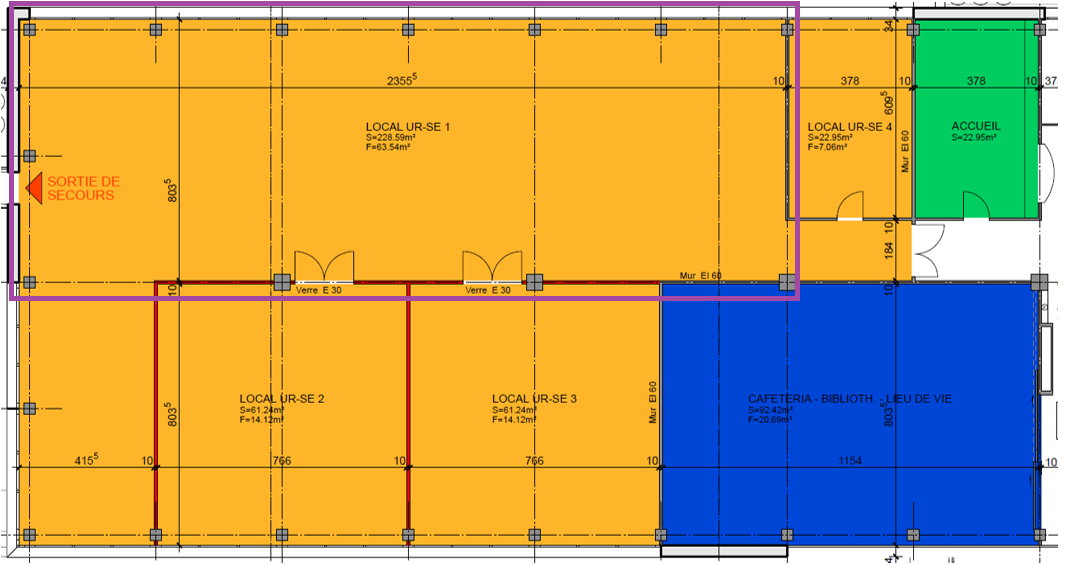
\includegraphics[scale=0.4]{figures/PlanRe.png}
		\caption{Plan réel de la salle}
		\label{fig:PlanRe} %% NOTE: always label *after* caption!
	\end{center}
\end{figure}

La figure \ref{fig:PlanRe} montre le plan modélisé et l'endroit où les mesures seront prises et le placement du maitre et des esclaves.
\begin{figure}[H]
	\begin{center}
		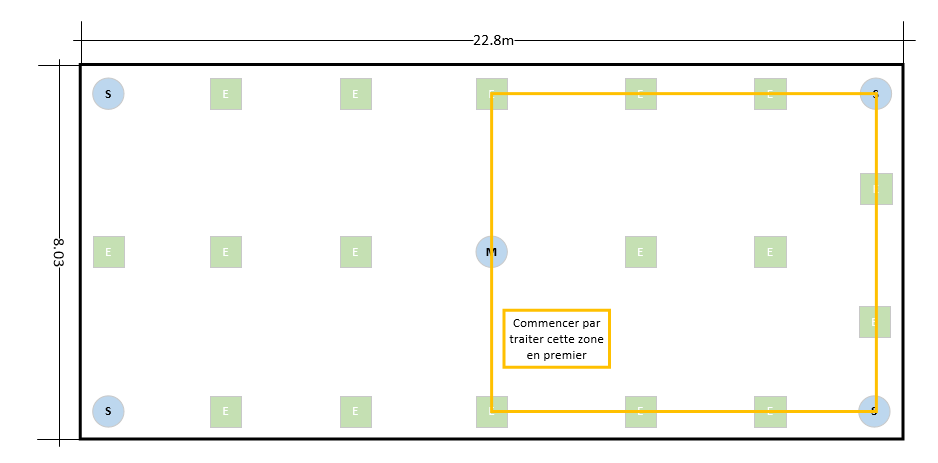
\includegraphics[scale=0.4]{figures/PlanMod.png}
		\caption{Plan indiquant l'endroit des mesures}
		\label{fig:PlanMod} %% NOTE: always label *after* caption!
	\end{center}
\end{figure}

\section{réflexions diverse}
Le choix de l'alforithme n'est pas chose aisée. Même de ssélectionner si on veut faire une régression ou une classification. La regression est quelque chose d'un peu plus compliqué et il est nécessaire d'avoir de très bonnes données ce que je ne sais pas actuellement. Je pense qu'il est préférable dans un premier temps de faire une classification et du coup de donne une zone de positionnement afin de traiter au mieux les datasets. Car le point le plus important c'est la prise de données et depuis la leur traitement. le choix de l'algorithme peut être choisi en fin de processus. 

Il y a possibilité de partir avec SVM pour la classification et ensuite SVR 
Ou alors même KNN pour la classification qui est pas mal cité dans les lectures et qui peut également être utilisé pour la regression.
Et finalement selon certain conseils et recherche concernant ce qui se fait l'algorithme randomforest peut être bien pour débuter car également il permet de faire de la classification ainsi que de la régression.

%\begin{enumerate}
%	\item fgfd
%	\item gdgfd
%\end{enumerate}


%\begin{figure}[H]
%	\begin{center}
%		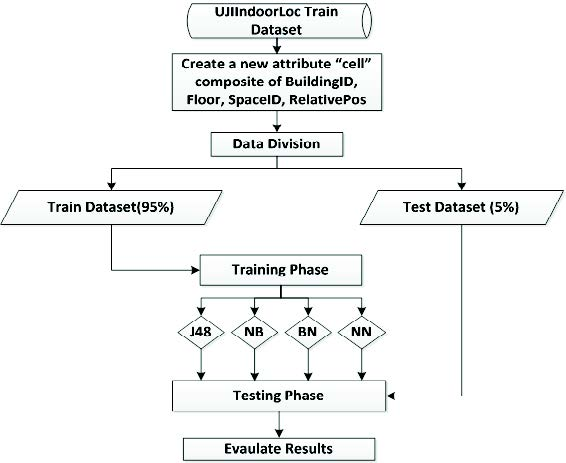
\includegraphics[scale=1]{figures/newattribute.jpg}
%		\caption{The new attribute “cell” construction phase}
%		\label{fig:newAttribute} %% NOTE: always label *after* caption!
%	\end{center}
%\end{figure}

%\todo{Compléter cette partie qui semble importante}
